% **************************************************************************************************************
% A Classic Thesis Style
% An Homage to The Elements of Typographic Style
%
% Copyright (C) 2017 André Miede and Ivo Pletikosić
%
% If you like the style then I would appreciate a postcard. My address
% can be found in the file ClassicThesis.pdf. A collection of the
% postcards I received so far is available online at
% http://postcards.miede.de
%
% License:
% This program is free software; you can redistribute it and/or modify
% it under the terms of the GNU General Public License as published by
% the Free Software Foundation; either version 2 of the License, or
% (at your option) any later version.
%
% This program is distributed in the hope that it will be useful,
% but WITHOUT ANY WARRANTY; without even the implied warranty of
% MERCHANTABILITY or FITNESS FOR A PARTICULAR PURPOSE.  See the
% GNU General Public License for more details.
%
% You should have received a copy of the GNU General Public License
% along with this program; see the file COPYING.  If not, write to
% the Free Software Foundation, Inc., 59 Temple Place - Suite 330,
% Boston, MA 02111-1307, USA.
% **************************************************************************************************************

\RequirePackage{silence}
\WarningFilter{scrreprt}{Usage of package `titlesec'}
\WarningFilter{titlesec}{Non standard sectioning command detected}
\documentclass[ twoside,openright,titlepage,numbers=noenddot,
                headinclude,footinclude,cleardoublepage=empty,
                BCOR=5mm,paper=a4,fontsize=11pt
                ]{scrreprt}

%********************************************************************
% Note: Make all your adjustments in here
%*******************************************************
% ****************************************************************************************************
% classicthesis-config.tex
% formerly known as loadpackages.sty, classicthesis-ldpkg.sty, and classicthesis-preamble.sty
% Use it at the beginning of your ClassicThesis.tex, or as a LaTeX Preamble
% in your ClassicThesis.{tex,lyx} with % ****************************************************************************************************
% classicthesis-config.tex
% formerly known as loadpackages.sty, classicthesis-ldpkg.sty, and classicthesis-preamble.sty
% Use it at the beginning of your ClassicThesis.tex, or as a LaTeX Preamble
% in your ClassicThesis.{tex,lyx} with % ****************************************************************************************************
% classicthesis-config.tex
% formerly known as loadpackages.sty, classicthesis-ldpkg.sty, and classicthesis-preamble.sty
% Use it at the beginning of your ClassicThesis.tex, or as a LaTeX Preamble
% in your ClassicThesis.{tex,lyx} with \input{classicthesis-config}
% ****************************************************************************************************
% If you like the classicthesis, then I would appreciate a postcard.
% My address can be found in the file ClassicThesis.pdf. A collection
% of the postcards I received so far is available online at
% http://postcards.miede.de
% ****************************************************************************************************


% ****************************************************************************************************
% 0. Set the encoding of your files. UTF-8 is the only sensible encoding nowadays. If you can't read
% äöüßáéçèê∂åëæƒÏ€ then change the encoding setting in your editor, not the line below. If your editor
% does not support utf8 use another editor!
% ****************************************************************************************************
\PassOptionsToPackage{utf8}{inputenc}
  \usepackage{inputenc}

% ****************************************************************************************************
% 1. Configure classicthesis for your needs here, e.g., remove "drafting" below
% in order to deactivate the time-stamp on the pages
% (see ClassicThesis.pdf for more information):
% ****************************************************************************************************
\PassOptionsToPackage{
  drafting=true,    % print version information on the bottom of the pages
  tocaligned=false, % the left column of the toc will be aligned (no indentation)
  dottedtoc=false,  % page numbers in ToC flushed right
  parts=true,       % use part division
  eulerchapternumbers=true, % use AMS Euler for chapter font (otherwise Palatino)
  linedheaders=false,       % chaper headers will have line above and beneath
  floatperchapter=true,     % numbering per chapter for all floats (i.e., Figure 1.1)
  eulermath=false,  % use awesome Euler fonts for mathematical formulae (only with pdfLaTeX)
  beramono=true,    % toggle a nice monospaced font (w/ bold)
  % palatino=false,   % deactivate standard font for loading another one, see the last section at the end of this file for suggestions
}{classicthesis}


% ****************************************************************************************************
% 2. Personal data and user ad-hoc commands
% ****************************************************************************************************
\newcommand{\myTitle}{Cathodic Protection Prediction\xspace}
\newcommand{\mySubtitle}{Time-series predictions with GMLVQ\xspace}
\newcommand{\myDegree}{Bachelor Information and Communication Technology (B.ICT)\xspace}
\newcommand{\myName}{Jelle van Wezel\xspace}
\newcommand{\myProf}{Michael Biehl\xspace}
\newcommand{\myOtherProf}{TBA\xspace}
\newcommand{\mySupervisor}{Richard Bosgraaf\xspace}
\newcommand{\myFaculty}{FWN\xspace}
\newcommand{\myDepartment}{Johannes Bernoulli Institute\xspace}
\newcommand{\myUni}{University of Groningen\xspace}
\newcommand{\myLocation}{Groningen\xspace}
\newcommand{\myTime}{May 2018\xspace}
\newcommand{\myVersion}{version 0.1}

% ********************************************************************
% Setup, finetuning, and useful commands
% ********************************************************************
\newcounter{dummy} % necessary for correct hyperlinks (to index, bib, etc.)
\newlength{\abcd} % for ab..z string length calculation
\providecommand{\mLyX}{L\kern-.1667em\lower.25em\hbox{Y}\kern-.125emX\@}
\newcommand{\ie}{i.\,e.}
\newcommand{\Ie}{I.\,e.}
\newcommand{\eg}{e.\,g.}
\newcommand{\Eg}{E.\,g.}
% ****************************************************************************************************


% ****************************************************************************************************
% 3. Loading some handy packages
% ****************************************************************************************************
% ********************************************************************
% Packages with options that might require adjustments
% ********************************************************************
\PassOptionsToPackage{american}{babel} % change this to your language(s), main language last
% Spanish languages need extra options in order to work with this template
%\PassOptionsToPackage{spanish,es-lcroman}{babel}
    \usepackage{babel}

\usepackage{csquotes}
\PassOptionsToPackage{%
  %backend=biber,bibencoding=utf8, %instead of bibtex
  backend=bibtex8,bibencoding=ascii,%
  language=auto,%
  style=numeric-comp,%
  %style=authoryear-comp, % Author 1999, 2010
  %bibstyle=authoryear,dashed=false, % dashed: substitute rep. author with ---
  sorting=nyt, % name, year, title
  maxbibnames=10, % default: 3, et al.
  %backref=true,%
  natbib=true % natbib compatibility mode (\citep and \citet still work)
}{biblatex}
    \usepackage{biblatex}

\PassOptionsToPackage{fleqn}{amsmath}       % math environments and more by the AMS
  \usepackage{amsmath}

% ********************************************************************
% General useful packages
% ********************************************************************
\PassOptionsToPackage{T1}{fontenc} % T2A for cyrillics
  \usepackage{fontenc}
\usepackage{textcomp} % fix warning with missing font shapes
\usepackage{scrhack} % fix warnings when using KOMA with listings package
\usepackage{xspace} % to get the spacing after macros right
\usepackage{mparhack} % get marginpar right
%\usepackage{fixltx2e} % fixes some LaTeX stuff --> since 2015 in the LaTeX kernel (see below)
% \usepackage[latest]{latexrelease} % emulate newer kernel version if older is detected
\PassOptionsToPackage{printonlyused,smaller}{acronym}
  \usepackage{acronym} % nice macros for handling all acronyms in the thesis
  %\renewcommand{\bflabel}[1]{{#1}\hfill} % fix the list of acronyms --> no longer working
  %\renewcommand*{\acsfont}[1]{\textsc{#1}}
  %\renewcommand*{\aclabelfont}[1]{\acsfont{#1}}
  %\def\bflabel#1{{#1\hfill}}
  \def\bflabel#1{{\acsfont{#1}\hfill}}
  \def\aclabelfont#1{\acsfont{#1}}
% ****************************************************************************************************
%\usepackage{pgfplots} % External TikZ/PGF support (thanks to Andreas Nautsch)
%\usetikzlibrary{external}
%\tikzexternalize[mode=list and make, prefix=ext-tikz/]
% ****************************************************************************************************


% ****************************************************************************************************
% 4. Setup floats: tables, (sub)figures, and captions
% ****************************************************************************************************
\usepackage{tabularx} % better tables
  \setlength{\extrarowheight}{3pt} % increase table row height
\newcommand{\tableheadline}[1]{\multicolumn{1}{l}{\spacedlowsmallcaps{#1}}}
\newcommand{\myfloatalign}{\centering} % to be used with each float for alignment
\usepackage{caption}
% Thanks to cgnieder and Claus Lahiri
% http://tex.stackexchange.com/questions/69349/spacedlowsmallcaps-in-caption-label
% [REMOVED DUE TO OTHER PROBLEMS, SEE ISSUE #82]
%\DeclareCaptionLabelFormat{smallcaps}{\bothIfFirst{#1}{~}\MakeTextLowercase{\textsc{#2}}}
%\captionsetup{font=small,labelformat=smallcaps} % format=hang,
\captionsetup{font=small} % format=hang,
\usepackage{subfig}
% ****************************************************************************************************


% ****************************************************************************************************
% 5. Setup code listings
% ****************************************************************************************************
\usepackage{listings}
%\lstset{emph={trueIndex,root},emphstyle=\color{BlueViolet}}%\underbar} % for special keywords
\lstset{language=[LaTeX]Tex,%C++,
  morekeywords={PassOptionsToPackage,selectlanguage},
  keywordstyle=\color{RoyalBlue},%\bfseries,
  basicstyle=\small\ttfamily,
  %identifierstyle=\color{NavyBlue},
  commentstyle=\color{Green}\ttfamily,
  stringstyle=\rmfamily,
  numbers=none,%left,%
  numberstyle=\scriptsize,%\tiny
  stepnumber=5,
  numbersep=8pt,
  showstringspaces=false,
  breaklines=true,
  %frameround=ftff,
  %frame=single,
  belowcaptionskip=.75\baselineskip
  %frame=L
}
% ****************************************************************************************************


% ****************************************************************************************************
% 6. PDFLaTeX, hyperreferences, and citation backreferences
% ****************************************************************************************************
% ********************************************************************
% Using PDFLaTeX
% ********************************************************************
\PassOptionsToPackage{hyperfootnotes=false,pdfpagelabels}{hyperref}
  \usepackage{hyperref}  % backref linktocpage pagebackref
  \usepackage{graphicx}


% ********************************************************************
% Hyperreferences
% ********************************************************************
\hypersetup{%
  %draft, % hyperref's draft mode, for printing see below
  colorlinks=true, linktocpage=true, pdfstartpage=3, pdfstartview=FitV,%
  % uncomment the following line if you want to have black links (e.g., for printing)
  %colorlinks=false, linktocpage=false, pdfstartpage=3, pdfstartview=FitV, pdfborder={0 0 0},%
  breaklinks=true, pdfpagemode=UseNone, pageanchor=true, pdfpagemode=UseOutlines,%
  plainpages=false, bookmarksnumbered, bookmarksopen=true, bookmarksopenlevel=1,%
  hypertexnames=true, pdfhighlight=/O,%nesting=true,%frenchlinks,%
  urlcolor=webbrown, linkcolor=RoyalBlue, citecolor=webgreen, %pagecolor=RoyalBlue,%
  %urlcolor=Black, linkcolor=Black, citecolor=Black, %pagecolor=Black,%
  pdftitle={\myTitle},%
  pdfauthor={\textcopyright\ \myName, \myUni, \myFaculty},%
  pdfsubject={},%
  pdfkeywords={},%
  pdfcreator={pdfLaTeX},%
  pdfproducer={LaTeX with hyperref and classicthesis}%
}

% ********************************************************************
% Setup autoreferences
% ********************************************************************
% There are some issues regarding autorefnames
% http://www.ureader.de/msg/136221647.aspx
% http://www.tex.ac.uk/cgi-bin/texfaq2html?label=latexwords
% you have to redefine the makros for the
% language you use, e.g., american, ngerman
% (as chosen when loading babel/AtBeginDocument)
% ********************************************************************
\makeatletter
\@ifpackageloaded{babel}%
  {%
    \addto\extrasamerican{%
      \renewcommand*{\figureautorefname}{Figure}%
      \renewcommand*{\tableautorefname}{Table}%
      \renewcommand*{\partautorefname}{Part}%
      \renewcommand*{\chapterautorefname}{Chapter}%
      \renewcommand*{\sectionautorefname}{Section}%
      \renewcommand*{\subsectionautorefname}{Section}%
      \renewcommand*{\subsubsectionautorefname}{Section}%
    }%
    \addto\extrasngerman{%
      \renewcommand*{\paragraphautorefname}{Absatz}%
      \renewcommand*{\subparagraphautorefname}{Unterabsatz}%
      \renewcommand*{\footnoteautorefname}{Fu\"snote}%
      \renewcommand*{\FancyVerbLineautorefname}{Zeile}%
      \renewcommand*{\theoremautorefname}{Theorem}%
      \renewcommand*{\appendixautorefname}{Anhang}%
      \renewcommand*{\equationautorefname}{Gleichung}%
      \renewcommand*{\itemautorefname}{Punkt}%
    }%
      % Fix to getting autorefs for subfigures right (thanks to Belinda Vogt for changing the definition)
      \providecommand{\subfigureautorefname}{\figureautorefname}%
    }{\relax}
\makeatother


% ****************************************************************************************************
% 7. Last calls before the bar closes
% ****************************************************************************************************
% ********************************************************************
% Development Stuff
% ********************************************************************
\listfiles
%\PassOptionsToPackage{l2tabu,orthodox,abort}{nag}
%  \usepackage{nag}
%\PassOptionsToPackage{warning, all}{onlyamsmath}
%  \usepackage{onlyamsmath}

% ********************************************************************
% Last, but not least...
% ********************************************************************
\usepackage{classicthesis}
% ****************************************************************************************************

\usepackage{wallpaper}

\newcommand{\placetextbox}[3]{% \placetextbox{<horizontal pos>}{<vertical pos>}{<stuff>}
  \setbox0=\hbox{#3}% Put <stuff> in a box
  \AddToShipoutPictureFG*{% Add <stuff> to current page foreground
    \put(\LenToUnit{#1\paperwidth},\LenToUnit{#2\paperheight}){\vtop{{\null}\makebox[0pt][c]{#3}}}%
  }%
}%


% ****************************************************************************************************
% 8. Further adjustments (experimental)
% ****************************************************************************************************
% ********************************************************************
% Changing the text area
% ********************************************************************
%\areaset[current]{312pt}{761pt} % 686 (factor 2.2) + 33 head + 42 head \the\footskip
%\setlength{\marginparwidth}{7em}%
%\setlength{\marginparsep}{2em}%

% ********************************************************************
% Using different fonts
% ********************************************************************
%\usepackage[oldstylenums]{kpfonts} % oldstyle notextcomp
% \usepackage[osf]{libertine}
%\usepackage[light,condensed,math]{iwona}
%\renewcommand{\sfdefault}{iwona}
%\usepackage{lmodern} % <-- no osf support :-(
%\usepackage{cfr-lm} %
%\usepackage[urw-garamond]{mathdesign} <-- no osf support :-(
%\usepackage[default,osfigures]{opensans} % scale=0.95
%\usepackage[sfdefault]{FiraSans}
% \usepackage[opticals,mathlf]{MinionPro} % onlytext
% ********************************************************************
%\usepackage[largesc,osf]{newpxtext}
%\linespread{1.05} % a bit more for Palatino
% Used to fix these:
% https://bitbucket.org/amiede/classicthesis/issues/139/italics-in-pallatino-capitals-chapter
% https://bitbucket.org/amiede/classicthesis/issues/45/problema-testatine-su-classicthesis-style
% ********************************************************************
% ****************************************************************************************************

% ****************************************************************************************************
% If you like the classicthesis, then I would appreciate a postcard.
% My address can be found in the file ClassicThesis.pdf. A collection
% of the postcards I received so far is available online at
% http://postcards.miede.de
% ****************************************************************************************************


% ****************************************************************************************************
% 0. Set the encoding of your files. UTF-8 is the only sensible encoding nowadays. If you can't read
% äöüßáéçèê∂åëæƒÏ€ then change the encoding setting in your editor, not the line below. If your editor
% does not support utf8 use another editor!
% ****************************************************************************************************
\PassOptionsToPackage{utf8}{inputenc}
  \usepackage{inputenc}

% ****************************************************************************************************
% 1. Configure classicthesis for your needs here, e.g., remove "drafting" below
% in order to deactivate the time-stamp on the pages
% (see ClassicThesis.pdf for more information):
% ****************************************************************************************************
\PassOptionsToPackage{
  drafting=true,    % print version information on the bottom of the pages
  tocaligned=false, % the left column of the toc will be aligned (no indentation)
  dottedtoc=false,  % page numbers in ToC flushed right
  parts=true,       % use part division
  eulerchapternumbers=true, % use AMS Euler for chapter font (otherwise Palatino)
  linedheaders=false,       % chaper headers will have line above and beneath
  floatperchapter=true,     % numbering per chapter for all floats (i.e., Figure 1.1)
  eulermath=false,  % use awesome Euler fonts for mathematical formulae (only with pdfLaTeX)
  beramono=true,    % toggle a nice monospaced font (w/ bold)
  % palatino=false,   % deactivate standard font for loading another one, see the last section at the end of this file for suggestions
}{classicthesis}


% ****************************************************************************************************
% 2. Personal data and user ad-hoc commands
% ****************************************************************************************************
\newcommand{\myTitle}{Cathodic Protection Prediction\xspace}
\newcommand{\mySubtitle}{Time-series predictions with GMLVQ\xspace}
\newcommand{\myDegree}{Bachelor Information and Communication Technology (B.ICT)\xspace}
\newcommand{\myName}{Jelle van Wezel\xspace}
\newcommand{\myProf}{Michael Biehl\xspace}
\newcommand{\myOtherProf}{TBA\xspace}
\newcommand{\mySupervisor}{Richard Bosgraaf\xspace}
\newcommand{\myFaculty}{FWN\xspace}
\newcommand{\myDepartment}{Johannes Bernoulli Institute\xspace}
\newcommand{\myUni}{University of Groningen\xspace}
\newcommand{\myLocation}{Groningen\xspace}
\newcommand{\myTime}{May 2018\xspace}
\newcommand{\myVersion}{version 0.1}

% ********************************************************************
% Setup, finetuning, and useful commands
% ********************************************************************
\newcounter{dummy} % necessary for correct hyperlinks (to index, bib, etc.)
\newlength{\abcd} % for ab..z string length calculation
\providecommand{\mLyX}{L\kern-.1667em\lower.25em\hbox{Y}\kern-.125emX\@}
\newcommand{\ie}{i.\,e.}
\newcommand{\Ie}{I.\,e.}
\newcommand{\eg}{e.\,g.}
\newcommand{\Eg}{E.\,g.}
% ****************************************************************************************************


% ****************************************************************************************************
% 3. Loading some handy packages
% ****************************************************************************************************
% ********************************************************************
% Packages with options that might require adjustments
% ********************************************************************
\PassOptionsToPackage{american}{babel} % change this to your language(s), main language last
% Spanish languages need extra options in order to work with this template
%\PassOptionsToPackage{spanish,es-lcroman}{babel}
    \usepackage{babel}

\usepackage{csquotes}
\PassOptionsToPackage{%
  %backend=biber,bibencoding=utf8, %instead of bibtex
  backend=bibtex8,bibencoding=ascii,%
  language=auto,%
  style=numeric-comp,%
  %style=authoryear-comp, % Author 1999, 2010
  %bibstyle=authoryear,dashed=false, % dashed: substitute rep. author with ---
  sorting=nyt, % name, year, title
  maxbibnames=10, % default: 3, et al.
  %backref=true,%
  natbib=true % natbib compatibility mode (\citep and \citet still work)
}{biblatex}
    \usepackage{biblatex}

\PassOptionsToPackage{fleqn}{amsmath}       % math environments and more by the AMS
  \usepackage{amsmath}

% ********************************************************************
% General useful packages
% ********************************************************************
\PassOptionsToPackage{T1}{fontenc} % T2A for cyrillics
  \usepackage{fontenc}
\usepackage{textcomp} % fix warning with missing font shapes
\usepackage{scrhack} % fix warnings when using KOMA with listings package
\usepackage{xspace} % to get the spacing after macros right
\usepackage{mparhack} % get marginpar right
%\usepackage{fixltx2e} % fixes some LaTeX stuff --> since 2015 in the LaTeX kernel (see below)
% \usepackage[latest]{latexrelease} % emulate newer kernel version if older is detected
\PassOptionsToPackage{printonlyused,smaller}{acronym}
  \usepackage{acronym} % nice macros for handling all acronyms in the thesis
  %\renewcommand{\bflabel}[1]{{#1}\hfill} % fix the list of acronyms --> no longer working
  %\renewcommand*{\acsfont}[1]{\textsc{#1}}
  %\renewcommand*{\aclabelfont}[1]{\acsfont{#1}}
  %\def\bflabel#1{{#1\hfill}}
  \def\bflabel#1{{\acsfont{#1}\hfill}}
  \def\aclabelfont#1{\acsfont{#1}}
% ****************************************************************************************************
%\usepackage{pgfplots} % External TikZ/PGF support (thanks to Andreas Nautsch)
%\usetikzlibrary{external}
%\tikzexternalize[mode=list and make, prefix=ext-tikz/]
% ****************************************************************************************************


% ****************************************************************************************************
% 4. Setup floats: tables, (sub)figures, and captions
% ****************************************************************************************************
\usepackage{tabularx} % better tables
  \setlength{\extrarowheight}{3pt} % increase table row height
\newcommand{\tableheadline}[1]{\multicolumn{1}{l}{\spacedlowsmallcaps{#1}}}
\newcommand{\myfloatalign}{\centering} % to be used with each float for alignment
\usepackage{caption}
% Thanks to cgnieder and Claus Lahiri
% http://tex.stackexchange.com/questions/69349/spacedlowsmallcaps-in-caption-label
% [REMOVED DUE TO OTHER PROBLEMS, SEE ISSUE #82]
%\DeclareCaptionLabelFormat{smallcaps}{\bothIfFirst{#1}{~}\MakeTextLowercase{\textsc{#2}}}
%\captionsetup{font=small,labelformat=smallcaps} % format=hang,
\captionsetup{font=small} % format=hang,
\usepackage{subfig}
% ****************************************************************************************************


% ****************************************************************************************************
% 5. Setup code listings
% ****************************************************************************************************
\usepackage{listings}
%\lstset{emph={trueIndex,root},emphstyle=\color{BlueViolet}}%\underbar} % for special keywords
\lstset{language=[LaTeX]Tex,%C++,
  morekeywords={PassOptionsToPackage,selectlanguage},
  keywordstyle=\color{RoyalBlue},%\bfseries,
  basicstyle=\small\ttfamily,
  %identifierstyle=\color{NavyBlue},
  commentstyle=\color{Green}\ttfamily,
  stringstyle=\rmfamily,
  numbers=none,%left,%
  numberstyle=\scriptsize,%\tiny
  stepnumber=5,
  numbersep=8pt,
  showstringspaces=false,
  breaklines=true,
  %frameround=ftff,
  %frame=single,
  belowcaptionskip=.75\baselineskip
  %frame=L
}
% ****************************************************************************************************


% ****************************************************************************************************
% 6. PDFLaTeX, hyperreferences, and citation backreferences
% ****************************************************************************************************
% ********************************************************************
% Using PDFLaTeX
% ********************************************************************
\PassOptionsToPackage{hyperfootnotes=false,pdfpagelabels}{hyperref}
  \usepackage{hyperref}  % backref linktocpage pagebackref
  \usepackage{graphicx}


% ********************************************************************
% Hyperreferences
% ********************************************************************
\hypersetup{%
  %draft, % hyperref's draft mode, for printing see below
  colorlinks=true, linktocpage=true, pdfstartpage=3, pdfstartview=FitV,%
  % uncomment the following line if you want to have black links (e.g., for printing)
  %colorlinks=false, linktocpage=false, pdfstartpage=3, pdfstartview=FitV, pdfborder={0 0 0},%
  breaklinks=true, pdfpagemode=UseNone, pageanchor=true, pdfpagemode=UseOutlines,%
  plainpages=false, bookmarksnumbered, bookmarksopen=true, bookmarksopenlevel=1,%
  hypertexnames=true, pdfhighlight=/O,%nesting=true,%frenchlinks,%
  urlcolor=webbrown, linkcolor=RoyalBlue, citecolor=webgreen, %pagecolor=RoyalBlue,%
  %urlcolor=Black, linkcolor=Black, citecolor=Black, %pagecolor=Black,%
  pdftitle={\myTitle},%
  pdfauthor={\textcopyright\ \myName, \myUni, \myFaculty},%
  pdfsubject={},%
  pdfkeywords={},%
  pdfcreator={pdfLaTeX},%
  pdfproducer={LaTeX with hyperref and classicthesis}%
}

% ********************************************************************
% Setup autoreferences
% ********************************************************************
% There are some issues regarding autorefnames
% http://www.ureader.de/msg/136221647.aspx
% http://www.tex.ac.uk/cgi-bin/texfaq2html?label=latexwords
% you have to redefine the makros for the
% language you use, e.g., american, ngerman
% (as chosen when loading babel/AtBeginDocument)
% ********************************************************************
\makeatletter
\@ifpackageloaded{babel}%
  {%
    \addto\extrasamerican{%
      \renewcommand*{\figureautorefname}{Figure}%
      \renewcommand*{\tableautorefname}{Table}%
      \renewcommand*{\partautorefname}{Part}%
      \renewcommand*{\chapterautorefname}{Chapter}%
      \renewcommand*{\sectionautorefname}{Section}%
      \renewcommand*{\subsectionautorefname}{Section}%
      \renewcommand*{\subsubsectionautorefname}{Section}%
    }%
    \addto\extrasngerman{%
      \renewcommand*{\paragraphautorefname}{Absatz}%
      \renewcommand*{\subparagraphautorefname}{Unterabsatz}%
      \renewcommand*{\footnoteautorefname}{Fu\"snote}%
      \renewcommand*{\FancyVerbLineautorefname}{Zeile}%
      \renewcommand*{\theoremautorefname}{Theorem}%
      \renewcommand*{\appendixautorefname}{Anhang}%
      \renewcommand*{\equationautorefname}{Gleichung}%
      \renewcommand*{\itemautorefname}{Punkt}%
    }%
      % Fix to getting autorefs for subfigures right (thanks to Belinda Vogt for changing the definition)
      \providecommand{\subfigureautorefname}{\figureautorefname}%
    }{\relax}
\makeatother


% ****************************************************************************************************
% 7. Last calls before the bar closes
% ****************************************************************************************************
% ********************************************************************
% Development Stuff
% ********************************************************************
\listfiles
%\PassOptionsToPackage{l2tabu,orthodox,abort}{nag}
%  \usepackage{nag}
%\PassOptionsToPackage{warning, all}{onlyamsmath}
%  \usepackage{onlyamsmath}

% ********************************************************************
% Last, but not least...
% ********************************************************************
\usepackage{classicthesis}
% ****************************************************************************************************

\usepackage{wallpaper}

\newcommand{\placetextbox}[3]{% \placetextbox{<horizontal pos>}{<vertical pos>}{<stuff>}
  \setbox0=\hbox{#3}% Put <stuff> in a box
  \AddToShipoutPictureFG*{% Add <stuff> to current page foreground
    \put(\LenToUnit{#1\paperwidth},\LenToUnit{#2\paperheight}){\vtop{{\null}\makebox[0pt][c]{#3}}}%
  }%
}%


% ****************************************************************************************************
% 8. Further adjustments (experimental)
% ****************************************************************************************************
% ********************************************************************
% Changing the text area
% ********************************************************************
%\areaset[current]{312pt}{761pt} % 686 (factor 2.2) + 33 head + 42 head \the\footskip
%\setlength{\marginparwidth}{7em}%
%\setlength{\marginparsep}{2em}%

% ********************************************************************
% Using different fonts
% ********************************************************************
%\usepackage[oldstylenums]{kpfonts} % oldstyle notextcomp
% \usepackage[osf]{libertine}
%\usepackage[light,condensed,math]{iwona}
%\renewcommand{\sfdefault}{iwona}
%\usepackage{lmodern} % <-- no osf support :-(
%\usepackage{cfr-lm} %
%\usepackage[urw-garamond]{mathdesign} <-- no osf support :-(
%\usepackage[default,osfigures]{opensans} % scale=0.95
%\usepackage[sfdefault]{FiraSans}
% \usepackage[opticals,mathlf]{MinionPro} % onlytext
% ********************************************************************
%\usepackage[largesc,osf]{newpxtext}
%\linespread{1.05} % a bit more for Palatino
% Used to fix these:
% https://bitbucket.org/amiede/classicthesis/issues/139/italics-in-pallatino-capitals-chapter
% https://bitbucket.org/amiede/classicthesis/issues/45/problema-testatine-su-classicthesis-style
% ********************************************************************
% ****************************************************************************************************

% ****************************************************************************************************
% If you like the classicthesis, then I would appreciate a postcard.
% My address can be found in the file ClassicThesis.pdf. A collection
% of the postcards I received so far is available online at
% http://postcards.miede.de
% ****************************************************************************************************


% ****************************************************************************************************
% 0. Set the encoding of your files. UTF-8 is the only sensible encoding nowadays. If you can't read
% äöüßáéçèê∂åëæƒÏ€ then change the encoding setting in your editor, not the line below. If your editor
% does not support utf8 use another editor!
% ****************************************************************************************************
\PassOptionsToPackage{utf8}{inputenc}
  \usepackage{inputenc}

% ****************************************************************************************************
% 1. Configure classicthesis for your needs here, e.g., remove "drafting" below
% in order to deactivate the time-stamp on the pages
% (see ClassicThesis.pdf for more information):
% ****************************************************************************************************
\PassOptionsToPackage{
  drafting=true,    % print version information on the bottom of the pages
  tocaligned=false, % the left column of the toc will be aligned (no indentation)
  dottedtoc=false,  % page numbers in ToC flushed right
  parts=true,       % use part division
  eulerchapternumbers=true, % use AMS Euler for chapter font (otherwise Palatino)
  linedheaders=false,       % chaper headers will have line above and beneath
  floatperchapter=true,     % numbering per chapter for all floats (i.e., Figure 1.1)
  eulermath=false,  % use awesome Euler fonts for mathematical formulae (only with pdfLaTeX)
  beramono=true,    % toggle a nice monospaced font (w/ bold)
  % palatino=false,   % deactivate standard font for loading another one, see the last section at the end of this file for suggestions
}{classicthesis}


% ****************************************************************************************************
% 2. Personal data and user ad-hoc commands
% ****************************************************************************************************
\newcommand{\myTitle}{Cathodic Protection Prediction\xspace}
\newcommand{\mySubtitle}{Time-series predictions with GMLVQ\xspace}
\newcommand{\myDegree}{Bachelor Information and Communication Technology (B.ICT)\xspace}
\newcommand{\myName}{Jelle van Wezel\xspace}
\newcommand{\myProf}{Michael Biehl\xspace}
\newcommand{\myOtherProf}{TBA\xspace}
\newcommand{\mySupervisor}{Richard Bosgraaf\xspace}
\newcommand{\myFaculty}{FWN\xspace}
\newcommand{\myDepartment}{Johannes Bernoulli Institute\xspace}
\newcommand{\myUni}{University of Groningen\xspace}
\newcommand{\myLocation}{Groningen\xspace}
\newcommand{\myTime}{May 2018\xspace}
\newcommand{\myVersion}{version 0.1}

% ********************************************************************
% Setup, finetuning, and useful commands
% ********************************************************************
\newcounter{dummy} % necessary for correct hyperlinks (to index, bib, etc.)
\newlength{\abcd} % for ab..z string length calculation
\providecommand{\mLyX}{L\kern-.1667em\lower.25em\hbox{Y}\kern-.125emX\@}
\newcommand{\ie}{i.\,e.}
\newcommand{\Ie}{I.\,e.}
\newcommand{\eg}{e.\,g.}
\newcommand{\Eg}{E.\,g.}
% ****************************************************************************************************


% ****************************************************************************************************
% 3. Loading some handy packages
% ****************************************************************************************************
% ********************************************************************
% Packages with options that might require adjustments
% ********************************************************************
\PassOptionsToPackage{american}{babel} % change this to your language(s), main language last
% Spanish languages need extra options in order to work with this template
%\PassOptionsToPackage{spanish,es-lcroman}{babel}
    \usepackage{babel}

\usepackage{csquotes}
\PassOptionsToPackage{%
  %backend=biber,bibencoding=utf8, %instead of bibtex
  backend=bibtex8,bibencoding=ascii,%
  language=auto,%
  style=numeric-comp,%
  %style=authoryear-comp, % Author 1999, 2010
  %bibstyle=authoryear,dashed=false, % dashed: substitute rep. author with ---
  sorting=nyt, % name, year, title
  maxbibnames=10, % default: 3, et al.
  %backref=true,%
  natbib=true % natbib compatibility mode (\citep and \citet still work)
}{biblatex}
    \usepackage{biblatex}

\PassOptionsToPackage{fleqn}{amsmath}       % math environments and more by the AMS
  \usepackage{amsmath}

% ********************************************************************
% General useful packages
% ********************************************************************
\PassOptionsToPackage{T1}{fontenc} % T2A for cyrillics
  \usepackage{fontenc}
\usepackage{textcomp} % fix warning with missing font shapes
\usepackage{scrhack} % fix warnings when using KOMA with listings package
\usepackage{xspace} % to get the spacing after macros right
\usepackage{mparhack} % get marginpar right
%\usepackage{fixltx2e} % fixes some LaTeX stuff --> since 2015 in the LaTeX kernel (see below)
% \usepackage[latest]{latexrelease} % emulate newer kernel version if older is detected
\PassOptionsToPackage{printonlyused,smaller}{acronym}
  \usepackage{acronym} % nice macros for handling all acronyms in the thesis
  %\renewcommand{\bflabel}[1]{{#1}\hfill} % fix the list of acronyms --> no longer working
  %\renewcommand*{\acsfont}[1]{\textsc{#1}}
  %\renewcommand*{\aclabelfont}[1]{\acsfont{#1}}
  %\def\bflabel#1{{#1\hfill}}
  \def\bflabel#1{{\acsfont{#1}\hfill}}
  \def\aclabelfont#1{\acsfont{#1}}
% ****************************************************************************************************
%\usepackage{pgfplots} % External TikZ/PGF support (thanks to Andreas Nautsch)
%\usetikzlibrary{external}
%\tikzexternalize[mode=list and make, prefix=ext-tikz/]
% ****************************************************************************************************


% ****************************************************************************************************
% 4. Setup floats: tables, (sub)figures, and captions
% ****************************************************************************************************
\usepackage{tabularx} % better tables
  \setlength{\extrarowheight}{3pt} % increase table row height
\newcommand{\tableheadline}[1]{\multicolumn{1}{l}{\spacedlowsmallcaps{#1}}}
\newcommand{\myfloatalign}{\centering} % to be used with each float for alignment
\usepackage{caption}
% Thanks to cgnieder and Claus Lahiri
% http://tex.stackexchange.com/questions/69349/spacedlowsmallcaps-in-caption-label
% [REMOVED DUE TO OTHER PROBLEMS, SEE ISSUE #82]
%\DeclareCaptionLabelFormat{smallcaps}{\bothIfFirst{#1}{~}\MakeTextLowercase{\textsc{#2}}}
%\captionsetup{font=small,labelformat=smallcaps} % format=hang,
\captionsetup{font=small} % format=hang,
\usepackage{subfig}
% ****************************************************************************************************


% ****************************************************************************************************
% 5. Setup code listings
% ****************************************************************************************************
\usepackage{listings}
%\lstset{emph={trueIndex,root},emphstyle=\color{BlueViolet}}%\underbar} % for special keywords
\lstset{language=[LaTeX]Tex,%C++,
  morekeywords={PassOptionsToPackage,selectlanguage},
  keywordstyle=\color{RoyalBlue},%\bfseries,
  basicstyle=\small\ttfamily,
  %identifierstyle=\color{NavyBlue},
  commentstyle=\color{Green}\ttfamily,
  stringstyle=\rmfamily,
  numbers=none,%left,%
  numberstyle=\scriptsize,%\tiny
  stepnumber=5,
  numbersep=8pt,
  showstringspaces=false,
  breaklines=true,
  %frameround=ftff,
  %frame=single,
  belowcaptionskip=.75\baselineskip
  %frame=L
}
% ****************************************************************************************************


% ****************************************************************************************************
% 6. PDFLaTeX, hyperreferences, and citation backreferences
% ****************************************************************************************************
% ********************************************************************
% Using PDFLaTeX
% ********************************************************************
\PassOptionsToPackage{hyperfootnotes=false,pdfpagelabels}{hyperref}
  \usepackage{hyperref}  % backref linktocpage pagebackref
  \usepackage{graphicx}


% ********************************************************************
% Hyperreferences
% ********************************************************************
\hypersetup{%
  %draft, % hyperref's draft mode, for printing see below
  colorlinks=true, linktocpage=true, pdfstartpage=3, pdfstartview=FitV,%
  % uncomment the following line if you want to have black links (e.g., for printing)
  %colorlinks=false, linktocpage=false, pdfstartpage=3, pdfstartview=FitV, pdfborder={0 0 0},%
  breaklinks=true, pdfpagemode=UseNone, pageanchor=true, pdfpagemode=UseOutlines,%
  plainpages=false, bookmarksnumbered, bookmarksopen=true, bookmarksopenlevel=1,%
  hypertexnames=true, pdfhighlight=/O,%nesting=true,%frenchlinks,%
  urlcolor=webbrown, linkcolor=RoyalBlue, citecolor=webgreen, %pagecolor=RoyalBlue,%
  %urlcolor=Black, linkcolor=Black, citecolor=Black, %pagecolor=Black,%
  pdftitle={\myTitle},%
  pdfauthor={\textcopyright\ \myName, \myUni, \myFaculty},%
  pdfsubject={},%
  pdfkeywords={},%
  pdfcreator={pdfLaTeX},%
  pdfproducer={LaTeX with hyperref and classicthesis}%
}

% ********************************************************************
% Setup autoreferences
% ********************************************************************
% There are some issues regarding autorefnames
% http://www.ureader.de/msg/136221647.aspx
% http://www.tex.ac.uk/cgi-bin/texfaq2html?label=latexwords
% you have to redefine the makros for the
% language you use, e.g., american, ngerman
% (as chosen when loading babel/AtBeginDocument)
% ********************************************************************
\makeatletter
\@ifpackageloaded{babel}%
  {%
    \addto\extrasamerican{%
      \renewcommand*{\figureautorefname}{Figure}%
      \renewcommand*{\tableautorefname}{Table}%
      \renewcommand*{\partautorefname}{Part}%
      \renewcommand*{\chapterautorefname}{Chapter}%
      \renewcommand*{\sectionautorefname}{Section}%
      \renewcommand*{\subsectionautorefname}{Section}%
      \renewcommand*{\subsubsectionautorefname}{Section}%
    }%
    \addto\extrasngerman{%
      \renewcommand*{\paragraphautorefname}{Absatz}%
      \renewcommand*{\subparagraphautorefname}{Unterabsatz}%
      \renewcommand*{\footnoteautorefname}{Fu\"snote}%
      \renewcommand*{\FancyVerbLineautorefname}{Zeile}%
      \renewcommand*{\theoremautorefname}{Theorem}%
      \renewcommand*{\appendixautorefname}{Anhang}%
      \renewcommand*{\equationautorefname}{Gleichung}%
      \renewcommand*{\itemautorefname}{Punkt}%
    }%
      % Fix to getting autorefs for subfigures right (thanks to Belinda Vogt for changing the definition)
      \providecommand{\subfigureautorefname}{\figureautorefname}%
    }{\relax}
\makeatother


% ****************************************************************************************************
% 7. Last calls before the bar closes
% ****************************************************************************************************
% ********************************************************************
% Development Stuff
% ********************************************************************
\listfiles
%\PassOptionsToPackage{l2tabu,orthodox,abort}{nag}
%  \usepackage{nag}
%\PassOptionsToPackage{warning, all}{onlyamsmath}
%  \usepackage{onlyamsmath}

% ********************************************************************
% Last, but not least...
% ********************************************************************
\usepackage{classicthesis}
% ****************************************************************************************************

\usepackage{wallpaper}

\newcommand{\placetextbox}[3]{% \placetextbox{<horizontal pos>}{<vertical pos>}{<stuff>}
  \setbox0=\hbox{#3}% Put <stuff> in a box
  \AddToShipoutPictureFG*{% Add <stuff> to current page foreground
    \put(\LenToUnit{#1\paperwidth},\LenToUnit{#2\paperheight}){\vtop{{\null}\makebox[0pt][c]{#3}}}%
  }%
}%


% ****************************************************************************************************
% 8. Further adjustments (experimental)
% ****************************************************************************************************
% ********************************************************************
% Changing the text area
% ********************************************************************
%\areaset[current]{312pt}{761pt} % 686 (factor 2.2) + 33 head + 42 head \the\footskip
%\setlength{\marginparwidth}{7em}%
%\setlength{\marginparsep}{2em}%

% ********************************************************************
% Using different fonts
% ********************************************************************
%\usepackage[oldstylenums]{kpfonts} % oldstyle notextcomp
% \usepackage[osf]{libertine}
%\usepackage[light,condensed,math]{iwona}
%\renewcommand{\sfdefault}{iwona}
%\usepackage{lmodern} % <-- no osf support :-(
%\usepackage{cfr-lm} %
%\usepackage[urw-garamond]{mathdesign} <-- no osf support :-(
%\usepackage[default,osfigures]{opensans} % scale=0.95
%\usepackage[sfdefault]{FiraSans}
% \usepackage[opticals,mathlf]{MinionPro} % onlytext
% ********************************************************************
%\usepackage[largesc,osf]{newpxtext}
%\linespread{1.05} % a bit more for Palatino
% Used to fix these:
% https://bitbucket.org/amiede/classicthesis/issues/139/italics-in-pallatino-capitals-chapter
% https://bitbucket.org/amiede/classicthesis/issues/45/problema-testatine-su-classicthesis-style
% ********************************************************************
% ****************************************************************************************************


%********************************************************************
% Bibliographies
%*******************************************************
\addbibresource{Bibliography.bib}
%********************************************************************
% Hyphenation
%*******************************************************
%\hyphenation{put special hyphenation here}

% ********************************************************************
% GO!GO!GO! MOVE IT!
%*******************************************************
\begin{document}
\frenchspacing
\raggedbottom
\selectlanguage{american}
%\renewcommand*{\bibname}{new name}
%\setbibpreamble{}
\pagenumbering{roman}
\pagestyle{plain}
%********************************************************************
% Frontmatter
%*******************************************************
\include{frontBackmatter/dirtyTitlepage}
%!TEX root = ../thesis.tex

%*******************************************************
% Titlepage
%*******************************************************
\begin{titlepage}

    \ThisULCornerWallPaper{1}{./gfx/front.jpg}
    \ThisULCornerWallPaper{0.15}{./gfx/rug_logo_white.png}
    \placetextbox{.5}{.4}{\Huge Cathodic Protection Prediction}
\end{titlepage}

%!TEX root = ../thesis.tex

\thispagestyle{empty}

\hfill

\vfill

\noindent\myName: \textit{\myTitle,} \mySubtitle, %\myDegree,
\textcopyright\ \myTime

%\bigskip
%
%\noindent\spacedlowsmallcaps{Supervisors}: \\
%\myProf \\
%\myOtherProf \\
%\mySupervisor
%
%\medskip
%
%\noindent\spacedlowsmallcaps{Location}: \\
%\myLocation
%
%\medskip
%
%\noindent\spacedlowsmallcaps{Time Frame}: \\
%\myTime

\cleardoublepage%!TEX root = ../thesis.tex

%*******************************************************
% Dedication
%*******************************************************
\thispagestyle{empty}
%\phantomsection
\refstepcounter{dummy}
\pdfbookmark[1]{Dedication}{Dedication}

\vspace*{3cm}

\begin{center}
    \emph{Ohana} means family. \\
    Family means nobody gets left behind, or forgotten. \\ \medskip
    --- Lilo \& Stitch
\end{center}

\medskip

\begin{center}
    Dedicated to the loving memory of Rudolf Miede. \\ \smallskip
    1939\,--\,2005
\end{center}

\cleardoublepage%!TEX root = ../thesis.tex

\pdfbookmark[1]{Foreword}{Foreword}
\begingroup

Foreword here \dots

\endgroup

\vfill
\cleardoublepage%!TEX root = ../thesis.tex

%*******************************************************
% Abstract
%*******************************************************

\pdfbookmark[1]{Abstract}{Abstract}
\begingroup
\let\clearpage\relax
\let\cleardoublepage\relax
\let\cleardoublepage\relax

\chapter*{Abstract}
Short summary of the contents in English\dots a great guide by
Kent Beck how to write good abstracts can be found here:
\begin{center}
\url{https://plg.uwaterloo.ca/~migod/research/beckOOPSLA.html}
\end{center}

\endgroup

\vfill

\cleardoublepage%!TEX root = ../thesis.tex

%*******************************************************
% Acknowledgments
%*******************************************************
\pdfbookmark[1]{Acknowledgments}{acknowledgments}

\begin{flushright}{\slshape
    We have seen that computer programming is an art, \\
    because it applies accumulated knowledge to the world, \\
    because it requires skill and ingenuity, and especially \\
    because it produces objects of beauty.} \\ \medskip
    --- \defcitealias{knuth:1974}{Donald E. Knuth}\citetalias{knuth:1974} \citep{knuth:1974}
\end{flushright}



\bigskip

\begingroup
\let\clearpage\relax
\let\cleardoublepage\relax
\let\cleardoublepage\relax
\chapter*{Acknowledgments}
Put your acknowledgments here.

Many thanks to everybody who already sent me a postcard!

Regarding the typography and other help, many thanks go to Marco
Kuhlmann, Philipp Lehman, Lothar Schlesier, Jim Young, Lorenzo
Pantieri and Enrico Gregorio\footnote{Members of GuIT (Gruppo
Italiano Utilizzatori di \TeX\ e \LaTeX )}, J\"org Sommer,
Joachim K\"ostler, Daniel Gottschlag, Denis Aydin, Paride
Legovini, Steffen Prochnow, Nicolas Repp, Hinrich Harms,
Roland Winkler, Jörg Weber, Henri Menke, Claus Lahiri,
Clemens Niederberger, Stefano Bragaglia, Jörn Hees,
Scott Lowe, Dave Howcroft, Jos\'e M. Alcaide, 
and the whole \LaTeX-community for support, ideas and
some great software.

\bigskip

\noindent\emph{Regarding \mLyX}: The \mLyX\ port was intially done by
\emph{Nicholas Mariette} in March 2009 and continued by
\emph{Ivo Pletikosi\'c} in 2011. Thank you very much for your
work and for the contributions to the original style.


\endgroup

\cleardoublepage%!TEX root = ../thesis.tex

%*******************************************************
% Table of Contents
%*******************************************************
\pagestyle{scrheadings}
%\phantomsection
\refstepcounter{dummy}
\pdfbookmark[1]{\contentsname}{tableofcontents}
\setcounter{tocdepth}{2} % <-- 2 includes up to subsections in the ToC
\setcounter{secnumdepth}{3} % <-- 3 numbers up to subsubsections
\manualmark
\markboth{\spacedlowsmallcaps{\contentsname}}{\spacedlowsmallcaps{\contentsname}}
\tableofcontents
\automark[section]{chapter}
\renewcommand{\chaptermark}[1]{\markboth{\spacedlowsmallcaps{#1}}{\spacedlowsmallcaps{#1}}}
\renewcommand{\sectionmark}[1]{\markright{\thesection\enspace\spacedlowsmallcaps{#1}}}
%*******************************************************
% List of Figures and of the Tables
%*******************************************************
\clearpage
% \pagestyle{empty} % Uncomment this line if your lists should not have any headlines with section name and page number
\begingroup
    \let\clearpage\relax
    \let\cleardoublepage\relax
    %*******************************************************
    % List of Figures
    %*******************************************************
    %\phantomsection
    \refstepcounter{dummy}
    %\addcontentsline{toc}{chapter}{\listfigurename}
    \pdfbookmark[1]{\listfigurename}{lof}
    \listoffigures

    \vspace{8ex}

    %*******************************************************
    % List of Tables
    %*******************************************************
    %\phantomsection
    \refstepcounter{dummy}
    %\addcontentsline{toc}{chapter}{\listtablename}
    \pdfbookmark[1]{\listtablename}{lot}
    \listoftables

    \vspace{8ex}
    % \newpage

    %*******************************************************
    % List of Listings
    %*******************************************************
    %\phantomsection
    \refstepcounter{dummy}
    %\addcontentsline{toc}{chapter}{\lstlistlistingname}
    \pdfbookmark[1]{\lstlistlistingname}{lol}
    \lstlistoflistings

    \vspace{8ex}

    %*******************************************************
    % Acronyms
    %*******************************************************
    %\phantomsection
    \refstepcounter{dummy}
    \pdfbookmark[1]{Acronyms}{acronyms}
    \markboth{\spacedlowsmallcaps{Acronyms}}{\spacedlowsmallcaps{Acronyms}}
    \chapter*{Acronyms}
    \begin{acronym}[UMLX]
        \acro{DRY}{Don't Repeat Yourself}
        \acro{API}{Application Programming Interface}
        \acro{UML}{Unified Modeling Language}
    \end{acronym}

\endgroup

%********************************************************************
% Mainmatter
%*******************************************************
\cleardoublepage
\pagestyle{scrheadings}
\pagenumbering{arabic}
%\setcounter{page}{90}
% use \cleardoublepage here to avoid problems with pdfbookmark
\cleardoublepage
%!TEX root = ../thesis.tex

\chapter{Introduction}\label{ch:introduction}

\section{Problem description}

Steel gas-pipes are placed in the ground where they form corrosion. The amount of formed corrosion is thought to be depending on multiple environment factors. For example, the composition of the soil, the ground water level, and the depth the pipes are placed. In order to prevent the formation of corrosion on the pipes a method called cathodic protection is applied. Cathodic protection uses an electrical system where anodes (metal rods) are placed in the ground near the cathode (the steel pipes). When current is introduced to the system corrosion forms on the anodes and not on the cathode. 

This method is applied on multiple pipe-lines by an energy company called `Cogas' which is located in Almelo. They have collected the environment factors by hand and know how much current is needed per pipe section. Because of the corrosion buildup over time on the anodes and the pipes, at some point in time the amount of current needed exceeds a threshold. At this point it is no longer possible or economically viable to produce the amount of current needed to prevent the corrosion. When this happens more anodes need to be placed or the steel pipes have to be replaced. Cogas wants to be able to predict when this will happen based on their collected data.

The project will be done for ValueA. ValueA provides ICT solutions for utility companies and has Cogas as a client. One of the software solutions ValueA has provided to Cogas is an interactive dashboard where pipe sections with some of their properties are shown. This project will focus on predicting when a pipe section needs maintenance by replacing the pipes or placing more anodes. These predictions could be incorporated in this dashboard.
It is unknown which environment factors (features) leads to the deterioration of the steel pipes. Methods like Supervised Variational Relevance Learning (SUVREL) and Global Metric Learning (GML) could give insight on which features are more important than others in this deterioration process. With the knowledge about the features predictions can be done on the dataset. For this project Learning Vector Quantization (LVQ) will be used to do the predictions. Its performance will be compared to the intuitive and widely used classifier K nearest neighbor (K-nn).

The cathodic protection predictions project is not the only project ValueA is involved with. Another classification problem involves Fraud detection in the energy grid. This problem forms the base of the graduation project of Sebastiaan van Loon. Since both the project of Sebastiaan van Loon and this project will be conducted at ValueA in the same period some collaboration will occur. This collaboration will consist of the development of an abstract module which includes an API that allows the existing software of ValueA to connect to a classifier implementing the abstract module.

This abstract module will be developed to ensure that the ValueA software can connect to a classification module independent of the methods the classification uses. This means that the development of the abstract module does not include the development of the actual classification algorithms and distance measures, which will be developed separately and are not part of the collaboration between Jelle van Wezel and Sebastiaan van Loon.

\section{Goals}

\begin{itemize}
\item Research existing techniques to map LVQ and KNN on a regression problem
\item Research existing methods for feature reduction/relevance
\item Develop a classification module for ValueA which can predict the lifespan of steel gas pipes with LVQ, KNN and a or multiple preprocessing methods like GML and SUVREL.
\item Offer a comparison of the results between the used methods
\item Describe the research, used methods, developed software, and the results.
\end{itemize}

\section{Working Environment}

The student will be partly embedded both in the Intelligent Systems research group within the JBI, and with ValueA at the location of Cogas, a customer of ValueA located in Almelo. It is envisioned that the student will work, on average, two days a week at Cogas and the remaining days at the university and at home. The student will have a meeting at least every fortnight with the first supervisor and will have at least one stand up a week with the third supervisor and/or other employees of ValueA and will attend the monthly meetings of the Intelligent Systems research group. 

The first and second supervisor will provide necessary expertise regarding the classification algorithms and dissimilarity measures used in the project. The third supervisor will provide necessary expertise about both the ValueA software solution and the energy utility market, provide data sets for the training and testing of the classifiers, and evaluate and offer feedback on the software developed.

The student will work on his own laptop and PC, and in case of failure work on a university managed system.  Deployment of software will be done on a cloud environment provided by ValueA. Code revisions will be stored in a GIT repository managed by ValueA. Data which ownership belongs to ValueA will remain in the ValueA cloud environment and will not be copied to the student’s laptops unless explicit permission is granted from ValueA.

\section{Deliverables}

As requested by ValueA the student will develop the software in Python.
\begin{itemize}
\item End of December. Classification module description. A document describing the classification module, its main features and its integration with the existing ValueA software.
\item Start of January. Literature survey. A document summarizing the main findings of a literature review and the relevant references regarding Cathodic protection predictions, LVQ, KNN, Metric learning.
\item End of January. Abstract classification module. An abstract module facilitating the connection of a classifier with the existing software and data of ValueA. (In collaboration with Sebastiaan van Loon.)
\item Mid of February. KNN classification module. A KNN classification module for predictions of gas pipe lifespan.
\item End of March. LVQ classification module. A LVQ module for predictions of gas pipe lifespan with relevance learning as initialization.
\item Mid of April. Test results.
\item Start of May. Thesis draft.
\item Mid of May. Presentation draft.
\item End of May. Presentation to the board of Cogas.
\item End of May. Final presentation, code, and thesis.
\end{itemize}
%!TEX root = ../thesis.tex

%************************************************
\chapter{Background}\label{ch:Background}
%************************************************

% RUG

% Cogas

% Pipe lines

% Coating

% Cathodic protection

%!TEX root = ../thesis.tex

\chapter{Pipeline Protection}\label{ch:pipeline-protection}


\section{Coating}

%Tell about coatings, pce and bitumen

% coating is the first layer of protection

% images of coatings

% costs of coating

% costs of maintenance

\section{Cathodic Protection}

% Cathodic Protection is second layer of protection

% Electorlyze

% Anode, chathode

% chemic reaction

% hydro-oxigen -> -800 mv

% Steel

% Lower thresh-hold

%!TEX root = ../thesis.tex

%************************************************
\chapter{Dataset}\label{ch:data}
%************************************************

\section{Configuration}
\label{sec:dataset:configuration}

The data consisted of 24 CP areas. Each of these areas have one anode point where the current is pushed into the ground. The current is then propagated through the ground and led back to the anode through the steel gas pipes completing the electric system.

The pipes spread from the anode and branch off from each-other, creating a tree like structure. The pipes are divided into segments, Usually where a pipe branches into two pipelines, two new segments form. A pipe can only be part of one segment but a segment can consist of multiple pipes. In between the segments measuring points are placed to measure the current and difference in voltages in the segment. The number of segments an measuring points differ per area and is shown in table %todo ref table.

% show table with the number of measuring points and segments per area.
\begin{table}[!htb]
\label{tab:dataset:measuring-points-per-area}
    \begin{minipage}{.5\textwidth}
        \centering
        \caption{}
        \label{tab:first}
        \begin{tabular}{rcl}
            right & center & left \\
            right & center & left 
        \end{tabular}
    \end{minipage}%
    \begin{minipage}{.5\textwidth}
        \centering
        \caption{}
        \label{tab:second}
        \begin{tabular}{rcl}
            right & center & left \\
            right & center & left 
        \end{tabular}
    \end{minipage}
\end{table}

%mep uit!!!!

\section{Missing Data}
\label{sec:dataset:missing-data}
Usually the measurements are conducted once per year at every measuring point. The measurements started as early as 1987 up-until 2016. This means their should be 39 measurements per measuring point. However this is not the case as is shown in figure  %todo ref figure

\begin{figure}[!htb]
\centering
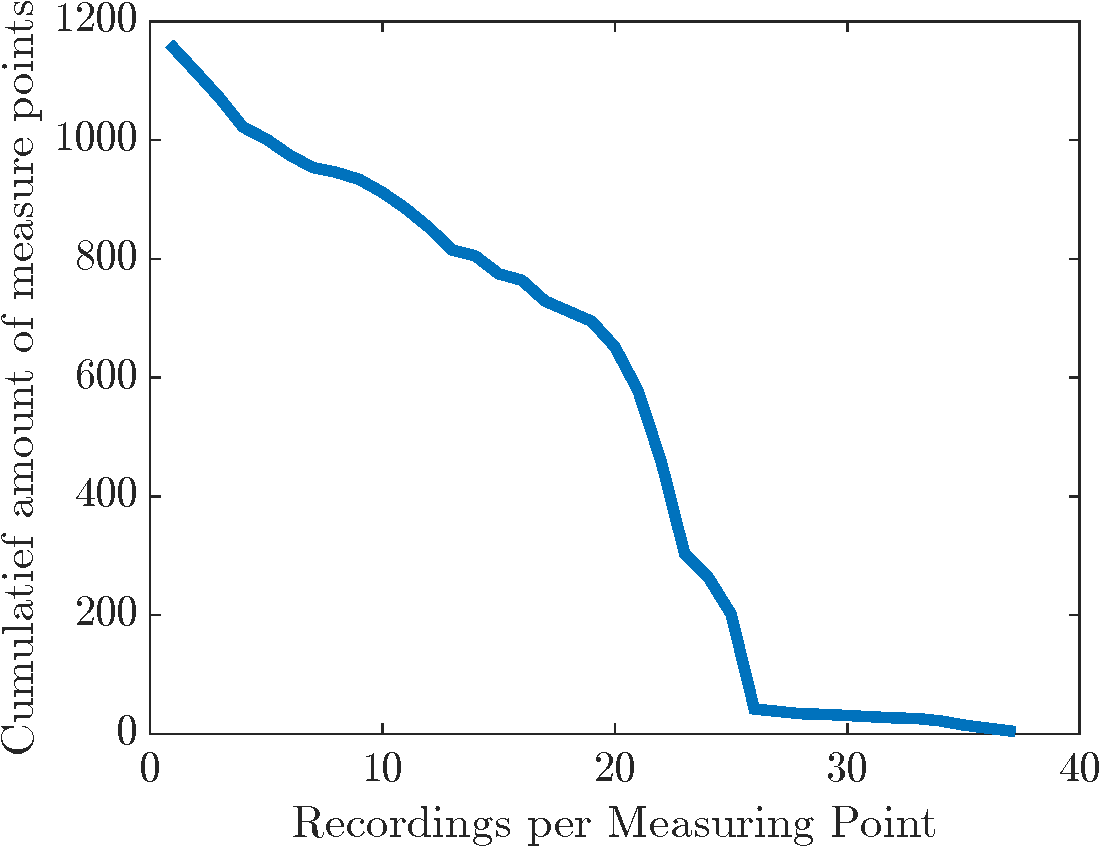
\includegraphics[width=.75\textwidth]{./gfx/chapters/data/cumulatief-recordings-per-measurepoint.pdf}
\caption{The number of measurements per measuring point against the cumulative number of measuring points having that number of measurements.}
\label{fig:dataset:cumulatief-recordings}
\end{figure}

Figure [REF] shows a fast drop in measurement points after the 20 measurements mark. At 26 measurements the drop stagnates and the maximum number of measurements is reached at 37 measurements. This means that none of the measuring points have the maximum number of 39 measurements.


% Tell about how the data was configured
% Show a figure with the tree, tell that it is a directed graph
% Tell about the different areas
% Tell about the measurepoints and that they have measurements

\section{Interpolation}
\label{sec:dataset:interpolation}
The method we proposed to use to predict the voltages of the pipelines with LVQ [REF] depends on the data being consistently spaced in time. 

Before the interpolation method was applied the data was checked for outliers by taking the mean and two times the standart deveation. Then removing the data points that did not fall in the range of $x > 2 \times \sigma - \mu$ and $x < 2 \times \sigma + \mu$.

\begin{figure}[!htb]
\centering
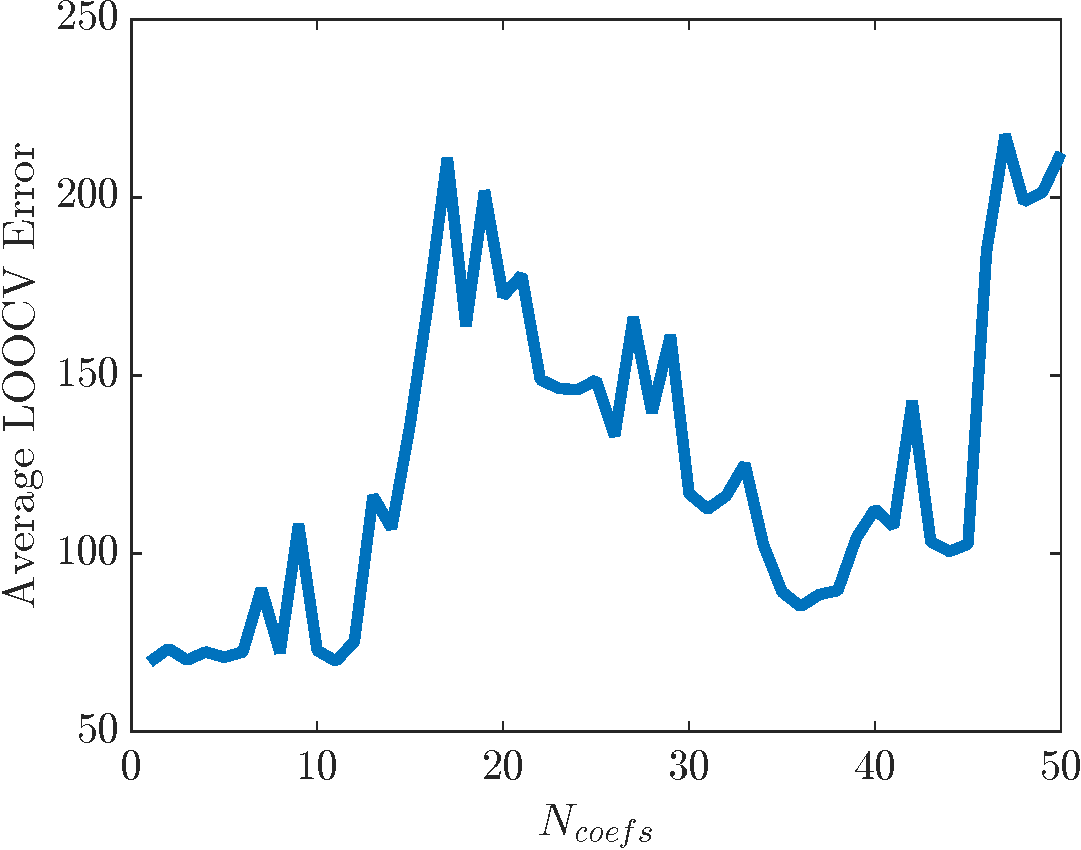
\includegraphics[width=.75\textwidth]{./gfx/chapters/data/Average-LOOCV-Error.pdf}
\caption{The average leave one out cross validation over all areas plotted against the number of $N$ coefficients used for the polynomial interpolation.}
\label{fig:dataset:cumulatief-recordings}
\end{figure}

% The data from the measuring points had many missing datapoints 
% The time (time-step) of the measurments was not concistent
% Used method to interpolate the data (show this in the method section)
% Describe the way this was done
% Leave One Out cross validation, to find an apropriate `n' (number of coeficients)
% Show the figure
% Describe the figure
% Tell the `n' should be 11 for reasons :D


%!TEX root = ../thesis.tex

%************************************************
\chapter{Methods}\label{ch:methods}
%************************************************


% Feature extraction

% 	Sliding window

% 	Coating

% 	Ground  Projections Amesfoort en intersections

%	Pipe Length

% Preprocessing

% 	Outlier removal

% 	Interpolation chebishev

% Classification

% 	LVQ
%	LGMLVQ
%	Linear regression
\section{Feature Extraction}

% queries -> measurements

% what features, 

% ground features, pipe features, how you did this with taking the bins.
% what are the bins of the features

% Projection of the areas and the pipes

% length of the pipes

% coating of the pipes

% average construction year of the pipes


\section{Preprocessing}

\section{Outlier removal}

% outlier removal 2*sd

\section{Chebishev}

% chebishev




\section{Classification}

\subsection{Learning Vector Quantization}

Learning vector quantization (LVQ) was introduced in the '90s by Kohonen \cite{kohonen} as a precursor to Self Organizing Maps (SOM). It is a prototype-based supervised classification algorithm. It uses a winner takes it all supervised Hebbian learning based approach. LVQ is defined by its prototypes often denoted as $W = (w_i , ... w_n)$. These prototypes are defined in the feature space of the dataset. Each epoch the algorithm iterates over the dataset and for each data-point it determines the closest prototype. The prototypes have labels from the same classes as the data-points. If the label of the prototype is the same as the label of the data-point, the prototype is updated by moving it in the direction of the data-point. If the labels differ, the prototype is moved away from the data-point. The distance a prototype travels is influenced by its location and a predetermined learning rate. The original heuristic has seen many variations since it was invented. The following sections go through the variations we used for classification on the datasets in this paper.

\subsection{Generalized Learning Vector Quantization}
\label{sssec:method:glvq}

The LVQ heuristic by Kohonen \cite{LVQ} needed proof of convergence, this was done by Sato and Yamada with Generalized Learning Vector Quantization (GLVQ) \cite{GLVQ}. They introduced an energy function $S$ based on the LVQ 2.1 scheme. Here there are two winning prototypes, one closest to the data-point with the same label as the data-point (denoted as $\vec{w}_J$) and the closest data-point with a different label, denoted by $\vec{w}_K$. Here $\vec{w}_J$ is moved towards the data-point and $\vec{w}_K$ is moved away from the data-point. They show that by optimizing the energy function through the prototypes this generalized version of LVQ always converges. The energy function is defined as 

\begin{flalign}
\label{eq:glvq-energy}
E = \sum_{i=1}^{P} \Phi(\mu(\vec{x}_i))\text{ , with }\mu(\vec{x}) = \frac{d_J-d_K}{d_J+d_K} \text{.}
\end{flalign}

The function, $\Phi(\mu)$, is monotonically increasing and $d_J$ and $d_K$ the squared distances from a data-point to the winning prototypes, defined by

\begin{flalign}
\label{eq:glvq-distance}
d_i = (\vec{x} - \vec{w}_i)^\top(\vec{x} - \vec{w}_i) \text{ , with } i=J,K \text{,}
\end{flalign}

\noindent with $\vec{x}$ the data-point and $\vec{w}_i$ one of the winning prototypes. The general update rule for the prototypes are defined by

\begin{flalign}
\label{eq:glvq-update-wi}
\Delta\vec{w}_i = - \alpha \frac{\partial E}{\partial \vec{w}_i} \text{ , with } i=J,K \text{,}
\end{flalign}

\noindent with $\alpha$ as the learning rate. Then based on equation \ref{eq:glvq-update-wi} the update rules for the prototypes are derived to be

\begin{flalign}
\label{eq:glvq-w1}
\Delta \vec{w}_J = \alpha \Phi'(\mu(\vec{x})) \frac{d_K}{(d_J+d_K)^2}(\vec{x}-\vec{w}_J) \text{,}
\end{flalign}

\begin{flalign}
\label{eq:glvq-w2}
\Delta \vec{w}_K = - \alpha \Phi'(\mu(\vec{x})) \frac{d_J}{(d_J+d_K)^2}(\vec{x}-\vec{w}_K) \text{.}
\end{flalign}

In equations \ref{eq:glvq-w1} and \ref{eq:glvq-w2} we can see prototype $\vec{w}_J$ is updated towards the data-point and prototype $\vec{w}_K$ is updated away from the data-point minimizing the energy function. The following LVQ methods (RGLVQ, GMLVQ, and LGMLVQ) are all based on this generalized variant of the LVQ 2.1 algorithm. In the experiments we only used these generalized versions of the LVQ algorithm. 

Because GLVQ uses a gradient descent (a stochastic gradient decent was used) to find an optimal location for its prototypes we used a fixed maximum iterations set to $2500$ for all variants of the algorithm. Furthermore the learning rate used was quadratically declining spread out over the number of iterations.

\subsubsection{Generalized Matrix Learning Vector Quantization}
%CITE GMLVQ
Generalized Matrix Learning Vector Quantization (GMLVQ) as proposed by Schneider et al. \cite{GMLVQ} uses a matrix $\Lambda$ instead of a vector (as in RGLVQ) to map the relevances and the combinations of the relevances between features. In order to gain a meaningful distance measure, $\Lambda$ has to be semi positive definite. This can be obtained by searching for the matrix $\Omega$ such that $\Lambda = \Omega^\top\Omega$. The method described here is based on the work by Schneider in her Ph.D. thesis \cite{Schneider}. The energy function for GMLVQ is written as

\begin{flalign}
E = \sum^P_{i=1}\Phi(\mu^\Lambda(\vec{x}_i)) \text{ , with } \mu^\Lambda(\vec{x}) = \frac{d^\Lambda_J-d^\Lambda_K}{d^\Lambda_J+d^\Lambda_K} \text{.}
\end{flalign}

Here the distance is influenced by the relevance matrix $\Lambda$ and defined as

\begin{flalign}
\label{eq:GMLVQ-distance}
d^\Lambda_i = (\vec{x} - \vec{w_i})^\top \Lambda (\vec{x} - \vec{w_i}) \text{, with } i=J,K \text{.}
\end{flalign}

Based on the energy function and this distance measure the new update rules are derived to

\begin{flalign}
\label{eq:GMLVQ-same-prototype}
\Delta \vec{w}_J = \alpha_1 \, \Phi' (\mu^\Lambda(\vec{x}))\, \mu^\Lambda_J(\vec{x})\, \Lambda \, (\vec{x} - \vec{w}_J) \text{,}
\end{flalign}

\begin{flalign}
\label{eq:GMLVQ-diff-prototype}
\Delta \vec{w}_K = - \alpha_1 \, \Phi' (\mu^\Lambda(\vec{x}))\, \mu^\Lambda_K(\vec{x})\, \Lambda \, (\vec{x} - \vec{w}_K) \text{.}
\end{flalign}

In these update rules $\alpha_1$ is the learning rate for the prototypes, $\mu^\Lambda_J(\vec{x})$ and $\mu^\Lambda_K(\vec{x})$ are defined as

\begin{flalign}
\mu^\Lambda_J(\vec{x}) = \frac{4d^\Lambda_K}{(d^\Lambda_J + d^\Lambda_K)^2} \text{,}
\end{flalign}

\begin{flalign}
\mu^\Lambda_K(\vec{x}) = \frac{4d^\Lambda_J}{(d^\Lambda_J + d^\Lambda_K)^2} \text{.}
\end{flalign}

 From the update rules in equations \ref{eq:GMLVQ-same-prototype} and \ref{eq:GMLVQ-diff-prototype}, the update rule for the matrix $\Omega$ is derived to
\begin{flalign}
\label{eq:GMLVQ-matrix-update}
\begin{split}
\Delta \Omega_{lm} =& - \alpha_2 \Phi' (\mu^\Lambda(\vec{x}))\\
&\Bigg(\mu^\Lambda_J(\vec{x}) \Big((x_m - w_{J,m})[\Omega(\vec{x}-\vec{w}_J)]_l\Big)\\
&-\mu^\Lambda_K(\vec{x}) \Big((x_m - w_{K,m})[\Omega(\vec{x}-\vec{w}_K)]_l\Big)\Bigg) \text{,}
\end{split}
\end{flalign}

where $\alpha_2$ is an independent learning rate from the learning rate $\alpha_1$ used in the update rules for the prototypes. After each update $\Lambda$ needs to be normalized (as with $\lambda$ in RGLVQ) to prevent GMLVQ from degeneration and this can be done by dividing all elements of $\Lambda$ by  $\sum_m\Lambda_{mm}$ and thus enforcing $\sum_m\Lambda_{mm} = 1$. This is a generalization for a simple diagonal metric of the normalization in GRLVQ where $\sum_m\lambda_{m} = 1$ was enforced.

\subsection{Localized Generalized Matrix Learning Vector Quantization}
%ref idk

The Localized GMLVQ (LGMLVQ) works with a more complex model using local matrices either attached to each prototype or in a class-wise manner. The update rules for the closest prototypes with the same and different labels are shown in equations \ref{eq:LGMLVQ-matrix-update-same} and \ref{eq:LGMLVQ-matrix-update-diff}.

\begin{flalign}
\label{eq:LGMLVQ-matrix-update-same}
\begin{split}
\Delta \Omega_{J,lm} =& - \alpha_2 \Phi' (\mu^\Lambda(\vec{x}))\\
&\mu^\Lambda_J(\vec{x}) \Big{(}(x_m - w_{J,m})[\Omega_J(\vec{x}-\vec{w}_J)]_l\Big{)} \text{,}
\end{split}
\end{flalign}

\begin{flalign}
\label{eq:LGMLVQ-matrix-update-diff}
\begin{split}
\Delta \Omega_{K,lm} =& + \alpha_2 \Phi' (\mu^\Lambda(\vec{x}))\\
&\mu^\Lambda_K(\vec{x}) \Big{(}(x_m - w_{K,m})[\Omega_K(\vec{x}-\vec{w}_K)]_l\Big{)} \text{.}
\end{split}
\end{flalign}

% short term long term predictions

% Linear regression

\section{Linear Regression}

\begin{flalign}
\label{eq:lin-reg}
y = \alpha + \beta
\end{flalign}

\begin{flalign}
\label{eq:lin-reg}
x = \bar y + \hat \beta \bar x
\end{flalign}

\begin{flalign}
\label{eq:lin-reg}
\bar y = \frac{1}{n} \sum_{i=1}^{n} y_i
\end{flalign}

\begin{flalign}
\label{eq:lin-reg}
\bar x = \frac{1}{n} \sum_{i=1}^{n} x_i
\end{flalign}

\begin{flalign}
\label{eq:lin-reg}
\begin{split}
\hat \beta &= \frac{\sum_{i=1}^{n} (x_i-\bar x)(y_i - \bar y)}{\sum_{i=1}^{n} (x_i-\bar x)^2}\\
&= \frac{\text{cov}(x,y)}{\text{var}(x)}
\end{split}
\end{flalign}

\section{R squared}

\begin{flalign}
\label{eq:lin-reg}
R^2 = 1  - \frac{\sum_{i=1}^{n}(y_i - \bar y)^2}{\sum_{i=1}^{n}(y_i - f_i)^2}
\end{flalign}

% Cross validation

% what parameters

% 

\include{chapters/experiments}
%!TEX root = ../thesis.tex

%************************************************
\chapter{Results}\label{ch:results}
%************************************************

% results cross validation chebishev

% results cross validation lvq

% results validation set

% show the eigen values of the matrici (find out what these entail)

% show the confusion matrici

% results linear regression

% show measurement of fitting on the linear regression and on the lvq long term predictions
%!TEX root = ../thesis.tex

%************************************************
\chapter{Discussion}\label{ch:discussion}
%************************************************
\include{chapters/conclusion}
% Backmatter
%*******************************************************
\appendix
\include{appendices/appendixA}
%********************************************************************
% Other Stuff in the Back
%*******************************************************
\cleardoublepage%!TEX root = ../thesis.tex

%********************************************************************
% Bibliography
%*******************************************************
% work-around to have small caps also here in the headline
% https://tex.stackexchange.com/questions/188126/wrong-header-in-bibliography-classicthesis
% Thanks to Enrico Gregorio
\defbibheading{bibintoc}[\bibname]{%
  \phantomsection
  \manualmark
  \markboth{\spacedlowsmallcaps{#1}}{\spacedlowsmallcaps{#1}}%
  \addtocontents{toc}{\protect\vspace{\beforebibskip}}%
  \addcontentsline{toc}{chapter}{\tocEntry{#1}}%
  \chapter*{#1}%
}
\printbibliography[heading=bibintoc]

% Old version, will be removed later
% work-around to have small caps also here in the headline
%\manualmark
%\markboth{\spacedlowsmallcaps{\bibname}}{\spacedlowsmallcaps{\bibname}} % work-around to have small caps also
%\phantomsection
%\refstepcounter{dummy}
%\addtocontents{toc}{\protect\vspace{\beforebibskip}} % to have the bib a bit from the rest in the toc
%\addcontentsline{toc}{chapter}{\tocEntry{\bibname}}
%\label{app:bibliography}
%\printbibliography

\cleardoublepage%!TEX root = ../thesis.tex

%*******************************************************
% Declaration
%*******************************************************
\refstepcounter{dummy}
\pdfbookmark[0]{Declaration}{declaration}
\chapter*{Declaration}
\thispagestyle{empty}
Put your declaration here.
\bigskip

\noindent\textit{\myLocation, \myTime}

\smallskip

\begin{flushright}
    \begin{tabular}{m{5cm}}
        \\ \hline
        \centering\myName \\
    \end{tabular}
\end{flushright}

\cleardoublepage%!TEX root = ../thesis.tex

\pagestyle{empty}

\hfill

\vfill


\pdfbookmark[0]{Colophon}{colophon}
\section*{Colophon}
This document was typeset using the typographical look-and-feel \texttt{classicthesis} developed by Andr\'e Miede and Ivo Pletikosić.
The style was inspired by Robert Bringhurst's seminal book on typography ``\emph{The Elements of Typographic Style}''.
\texttt{classicthesis} is available for both \LaTeX\ and \mLyX:
\begin{center}
\url{https://bitbucket.org/amiede/classicthesis/}
\end{center}
Happy users of \texttt{classicthesis} usually send a real postcard to the author, a collection of postcards received so far is featured here:
\begin{center}
\url{http://postcards.miede.de/}
\end{center}
Thank you very much for your feedback and contribution.

\bigskip

\noindent\finalVersionString

%Hermann Zapf's \emph{Palatino} and \emph{Euler} type faces (Type~1 PostScript fonts \emph{URW
%Palladio L} and \emph{FPL}) are used. The ``typewriter'' text is typeset in \emph{Bera Mono},
%originally developed by Bitstream, Inc. as ``Bitstream Vera''. (Type~1 PostScript fonts were made
%available by Malte Rosenau and
%Ulrich Dirr.)

%\paragraph{note:} The custom size of the textblock was calculated
%using the directions given by Mr. Bringhurst (pages 26--29 and
%175/176). 10~pt Palatino needs  133.21~pt for the string
%``abcdefghijklmnopqrstuvwxyz''. This yields a good line length between
%24--26~pc (288--312~pt). Using a ``\emph{double square textblock}''
%with a 1:2 ratio this results in a textblock of 312:624~pt (which
%includes the headline in this design). A good alternative would be the
%``\emph{golden section textblock}'' with a ratio of 1:1.62, here
%312:505.44~pt. For comparison, \texttt{DIV9} of the \texttt{typearea}
%package results in a line length of 389~pt (32.4~pc), which is by far
%too long. However, this information will only be of interest for
%hardcore pseudo-typographers like me.%
%
%To make your own calculations, use the following commands and look up
%the corresponding lengths in the book:
%\begin{verbatim}
%    \settowidth{\abcd}{abcdefghijklmnopqrstuvwxyz}
%    \the\abcd\ % prints the value of the length
%\end{verbatim}
%Please see the file \texttt{classicthesis.sty} for some precalculated
%values for Palatino and Minion.
%
%    \settowidth{\abcd}{abcdefghijklmnopqrstuvwxyz}
%    \the\abcd\ % prints the value of the length

% ********************************************************************
% Game Over: Restore, Restart, or Quit?
%*******************************************************
\end{document}
% ********************************************************************
